\chapter{Grundlagen}\label{ch:foundation}


\section{Microservice Architektur}\label{sec:foundation_microservices}

Die Microservice-Architektur ist ein Architekturstil für die Softwareentwicklung, bei dem eine Anwendung als eine Sammlung unabhängiger, kleiner Dienste aufgebaut wird.
Jeder dieser Dienste ist eigenständig und erfüllt eine spezifische Geschäftsanforderung.
Diese Architektur hat sich als Alternative zur monolithischen Architektur etabliert, bei der alle Funktionalitäten einer Anwendung in einer einzigen, großen Codebasis zusammengefasst sind.

Ein wesentliches Merkmal der Microservice-Architektur ist die Unabhängigkeit der Dienste.
Jeder Microservice kann eigenständig entwickelt, getestet, bereitgestellt und skaliert werden.
Die lose Kopplung zwischen den Diensten wird durch wohl definierte \glspl{API} sichergestellt, die häufig auf REST
oder Messaging-Protokollen basieren~\cite{richardsonMicroservicesPatterns2018}.
Zudem wird die funktionale Trennung betont, da jeder Service einen klar definierten Anwendungsteil abdeckt und von einem eigenen Entwicklungsteam verwaltet werden kann.
Diese Struktur ermöglicht es, unterschiedliche Technologien oder Programmiersprachen für verschiedene Services einzusetzen, wodurch eine technologische Vielfalt innerhalb eines Systems entsteht.
So entstehen mehrere kleine Anwendungen, die einfacher zu verstehen und zu warten sind als ein großer
Technologie-Stack wie in einer monolithischen Architektur.

Die Microservice-Architektur bietet zahlreiche Vorteile.
Sie ermöglicht eine hohe Flexibilität, da Änderungen an einem Service unabhängig von anderen vorgenommen werden können.
Die Fehlertoleranz wird verbessert, da ein Fehler in einem Microservice nicht zwangsläufig die gesamte Anwendung beeinträchtigt.
Durch die gezielte Bereitstellung von Ressourcen für bestimmte Dienste kann die Skalierbarkeit optimiert werden.
Zudem erleichtert die überschaubare Größe einzelner Microservices deren Wartung, da der Code besser verständlich und weniger komplex ist.

Trotz ihrer Vorteile bringt die Microservice-Architektur auch Herausforderungen mit sich.
Die Kommunikation zwischen den einzelnen Diensten erfordert robuste Schnittstellen und ein zuverlässiges \gls{API}-Management, um eine reibungslose Interaktion zu gewährleisten.
Die Verwaltung von Daten kann komplex sein, da die Konsistenz zwischen verschiedenen Microservices sichergestellt
werden muss.
Darüber hinaus erfordert die Vielzahl kleiner Dienste leistungsfähige Deployment- und Monitoring-Tools, um deren Verwaltung effizient zu gestalten.

Die Microservice-Architektur bildet die Grundlage für moderne verteilte Systeme und spielt eine zentrale Rolle für Cloud-Umgebungen.
Da bei dieser Architektur die Kommunikation zwischen den einzelnen Diensten im Vordergrund steht, ist eine zuverlässige Validierung der Schnittstellen essenziell.


\section{Testautomatisierung}\label{sec:foundation_testautomation}

Mit dem zunehmenden Bedarf an schneller Softwareauslieferung bei gleichbleibend hoher Qualität hat sich die Testautomatisierung zu einem zentralen Bestandteil moderner Entwicklungsprozesse entwickelt.
Sie beschreibt die automatisierte und kontinuierliche Durchführung von Tests, meist mithilfe spezialisierter Tools und Skripte, um manuelle Testaufwände zu reduzieren, Wiederholbarkeit zu gewährleisten und Fehler frühzeitig im Entwicklungsprozess zu erkennen.

Solche Praktiken und Tools werden häufig under dem Begriff \gls{DevOps} zusammengefasst.
\gls{DevOps} beschreibt eine kulturelle und technische Bewegung, die darauf abzielt, die Zusammenarbeit zwischen Entwicklungs- und Betriebsteams zu verbessern.
Ziel ist es, den gesamten Software-Lebenszyklus zu optimieren, von der Entwicklung über das Testing bis hin zum \gls{Deployment} und Betrieb.
Dazu zählen Dinge wie Kollaboration zwischen Teams, Automatisierung von regelmäßigen Aufgaben, Überwachung von
Anwendungsinfrastruktur und Auswertung von Nutzerfeedback.
%TODO: "Dinge" austauschen

Einige dieser Automatisierungen werden unter dem Begriff \gls{CI} zusammengefasst.
Das bedeutet, dass Änderungen am Code kontinuierlich in das gemeinsame Repository integriert werden und dabei
automatisierte \glspl{Build} und Tests ausgeführt werden, um sicherzustellen, dass der neue Code keine bestehenden
Funktionalitäten bricht.
Durch diese sofortige Rückmeldung können Fehler frühzeitig erkannt und behoben werden.

\Gls{CD} geht noch einen Schritt weiter: Nach der erfolgreichen Integration und dem Bestehen aller Tests wird die
Anwendung automatisiert für die Auslieferung vorbereitet und zusammengebaut.
Dies schließt Prozesse wie das Verpacken, Bereitstellen und Testen der Anwendung in produktionsnahen Umgebungen ein.
In der weitergehenden Form, dem sogenannten Continuous Deployment, erfolgt sogar die automatische Auslieferung in die Produktionsumgebung.

Testautomatisierung ist dabei das Rückgrat dieser Abläufe.
Sie ermöglicht nicht nur die schnelle und zuverlässige Durchführung von Unit-, Integrations- oder End-to-End-Tests, sondern auch die Validierung nichtfunktionaler Anforderungen wie Performance oder Sicherheit.
Diese Automatisierungen werden mithilfe von \gls{CI}/\gls{CD}-Pipelines orchestriert, die den gesamten Prozess von der Codeänderung bis zur Bereitstellung steuern.

Gerade in Microservice-Architekturen ist die Testautomatisierung unverzichtbar, da hier viele unabhängige Komponenten miteinander interagieren.
Ohne automatisierte Tests würde das Risiko fehlerhafter Integrationen oder regressiver Effekte drastisch steigen.
Contract Testing, als spezieller Ansatz innerhalb der Testautomatisierung, fokussiert sich gezielt auf die Kommunikation zwischen Microservices und stellt sicher, dass Änderungen in einem Dienst keine ungewollten Auswirkungen auf andere haben.

Insgesamt trägt Testautomatisierung in Verbindung mit \gls{DevOps} und \gls{CI}/\gls{CD} entscheidend dazu bei, die Qualität, Sicherheit und Stabilität moderner Softwareprodukte zu gewährleisten.


\section{Arten des Softwaretests}\label{sec:foundation_testing}

Um die Qualität und Funktionsfähigkeit von Software sicherzustellen, kommen verschiedene Arten von Softwaretests zum Einsatz.
Diese lassen sich nach ihrem Fokus und ihrer Testtiefe kategorisieren.

Unit-Tests (Modultests) überprüfen einzelne Funktionseinheiten, wie Funktionen oder Methoden, isoliert von anderen Komponenten.
Sie dienen dazu, die korrekte Implementierung kleinster funktionaler Einheiten sicherzustellen.
Hierbei sollten möglichst viele Einheiten getestet werden, um eine hohe Testabdeckung zu erreichen.
Wegen der verhältnismäßig gering Ausführungszeit kann
\textquote{[deren] Durchführung [\dots] sehr schnell, beliebig oft und aufwandsarm erfolgen}~\cite{linzBasiswissenSoftwaretest2024}.
Diese Tests sind in der Regel maschinell und werden häufig während der Entwicklung durchgeführt, um Fehler
frühzeitig zu erkennen.

Integrationstests hingegen testen das Zusammenspiel mehrerer Module oder Systeme.
Sie prüfen, ob die verschiedenen Komponenten korrekt miteinander interagieren.
Integrationstests sind wichtig, um sicherzustellen, dass die einzelnen Module nicht nur isoliert, sondern auch in Kombination miteinander funktionieren.
Die Testumgebung ist hierbei oft komplexer, da mehrere Module gleichzeitig zur Verfügung stehen müssen und somit ist
auch die Laufzeit höher.

Systemtests betrachten die Anwendung als Ganzes.
Dabei wird überprüft, ob das gesamte System konform zu den Anforderungen funktioniert.
Diese Tests sind in der Regel sehr umfangreich in der Erstellung und Ausführung, da sie alle Komponenten und deren Interaktionen berücksichtigen.
Darum sollten nur wenige Testfälle erstellt werden, die jedoch alle wichtigen Aspekte der Anwendung abdecken.

Akzeptanztests bilden die höchste Testebene und stellen sicher, dass die Anwendung aus Sicht der Endbenutzer den definierten Anforderungen entspricht.
Diese Tests werden häufig manuell und in enger Abstimmung mit den Stakeholdern durchgeführt~\cite{singhSoftwareTesting2011}.
Sie sind entscheidend für die Validierung der Software und deren Akzeptanz durch die Benutzer.
Aufgrund des hohen Aufwands sind diese Tests nicht Teil von Entwicklungszyklen, sondern werden in der Regel erst nach der Fertigstellung des Systems durchgeführt.

Die Hierarchie der verschiedenen Teststufen wird in~\cref{fig:testpyramid} dargestellt und verdeutlicht.

\begin{figure}[ht]
    \centering
    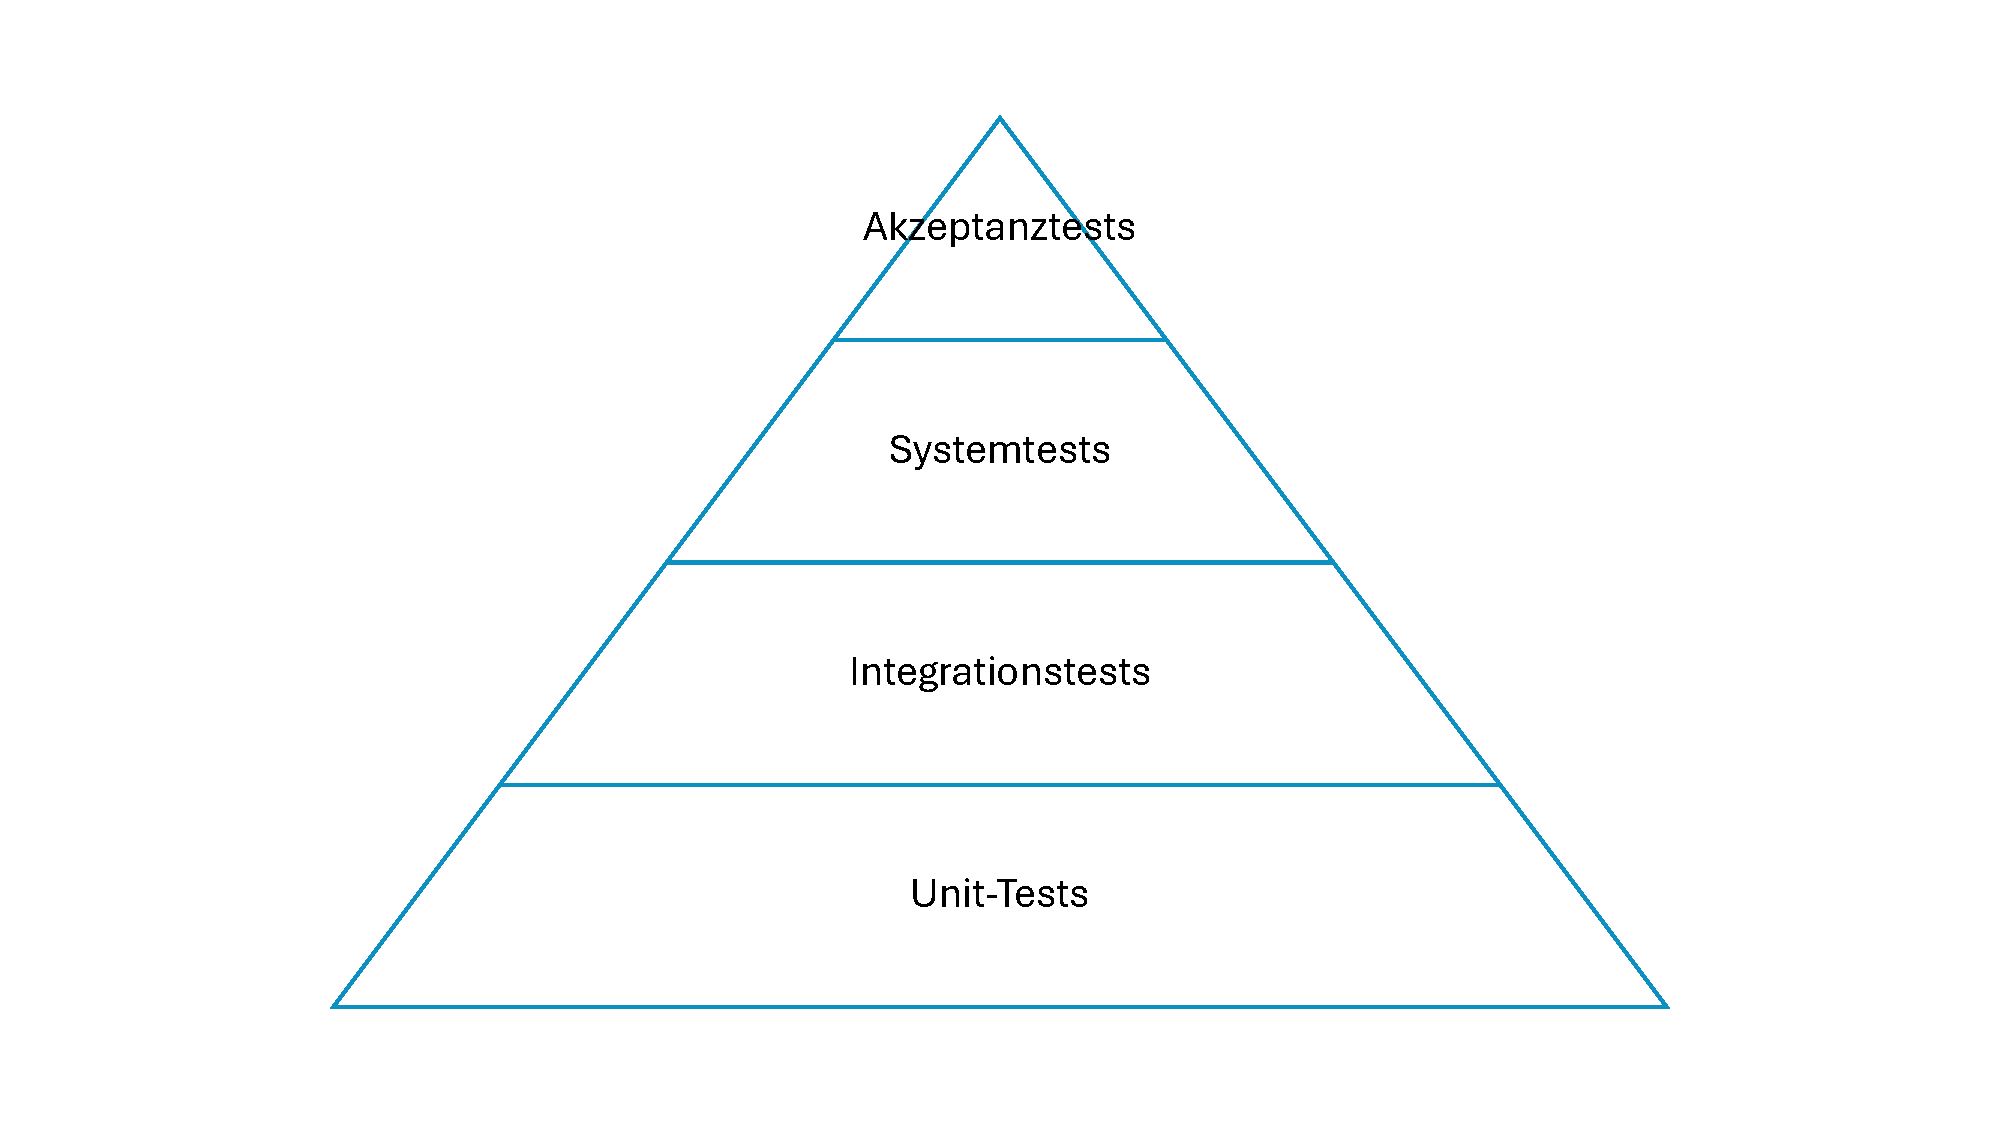
\includegraphics[width=0.8\textwidth]{figures/Testpyramide}
    \caption{Testpyramide nach \cite{linzBasiswissenSoftwaretest2024}}
    \label{fig:testpyramid}
\end{figure}

Neben diesen klassischen Testarten gibt es auch spezialisierte Testmethoden wie Performance-Tests, Sicherheitstests und Usability-Tests.
Diese Tests konzentrieren sich auf spezifische Aspekte der Softwarequalität und sind darauf ausgelegt, bestimmte Anforderungen zu validieren.
Deshalb sind diese nicht in die Testhierarchie der Testpyramide eingeordnet, sondern ergänzen diese.

Im Kontext von Microservices gewinnen automatisierte Tests und insbesondere Contract Tests an Bedeutung, da sie die Kommunikation zwischen Diensten absichern und frühzeitig Fehler in der Interaktion erkennen lassen.


\section{Contract Testing}\label{sec:foundation_contracttesting}

Contract Testing ist eine Testmethode, die darauf abzielt, die Interoperabilität zwischen verschiedenen Schnittstellen zu gewährleisten.
Während immer ofter Microservices Architekturen eingesetzt werden und Anwendungen aus vielen kleinen, unabhängigen Diensten bestehen, ist es wichtig das Zusammenspiel dieser Dienste zu testen.
Contract Testing kombiniert die Funktion von \gls{API}-Integrationstests mit der Zuverlässigkeit und Schnelligkeit von Unit-Tests und kann so Fehler bei der Schnittstellenkommunikation früher im Entwicklungsprozess erkennen~\cite{cruzContractTestingAction2025}.

\subsection{Funktionsweise}\label{subsec:foundation_contracttesting_concept}

Bei der Kommunikation mit \glspl{API} sind immer zwei Parteien beteiligt.
Zum einen gibt es einen Anbieter (Provider), der die Schnittstelle bereitstellt, und zum anderen einen bis mehrere Verbraucher (Consumer), die diese Schnittstelle nutzen. %TODO: Singular oder Plural bei Verbraucher?
Wenn ein Verbraucherdienst eine Schnittstelle ansprechen möchte, sendet er eine Anfrage an die \gls{API} des Anbieters.
Der Anbieter verarbeitet diese Anfrage, führt eventuelle zugehörige Aktionen aus und sendet eine Antwort zurück.
Auf der Verbraucherseite wird die Antwort bei Erhalt verarbeitet, um die gewünschten Informationen zu extrahieren und zu verwenden.
Um diese Verarbeitung zu ermöglichen, muss der Consumer eine Annahme über die Struktur der Antwort treffen.
In einer idealen Welt würde die Antwort immer der Struktur entsprechen, die der Consumer erwartet, doch das kann in der Praxis nicht immer garantiert werden.
Contract Testing sorgt dafür, dass diese Annahmen auch tatsächlich erfüllt werden und somit Fehler in der Kommunikation zwischen den Diensten vermieden werden.

Dabei wird ein sogenannter „Contract“ definiert – ein Vertrag, der beschreibt, wie die Kommunikation zwischen Consumer und Provider ablaufen soll.
Dieser Vertrag legt fest, welche Anfragen der Consumer an den Provider stellt und welche Antworten er im Gegenzug erwartet.
Der entscheidende Vorteil dabei ist, dass beide Seiten unabhängig voneinander testen können, ob sie diesen Vertrag einhalten.
Beim Contract Testing wird der Fokus also nicht auf die vollständige Funktionalität des Systems gelegt, sondern auf die Schnittstelle und die Erwartungen, die damit einhergehen.
Der Consumer beschreibt zunächst in Form eines Contracts, welche \gls{API}-Aufrufe er macht und wie die Antworten strukturiert sein sollen.
Dieser Contract wird anschließend verwendet, um automatisierte Tests sowohl auf Consumer- als auch auf Provider-Seite durchzuführen.

Auf der Consumer-Seite wird überprüft, ob die Anwendung tatsächlich nur die im Contract beschriebenen Anforderungen stellt.
Auf der Provider-Seite hingegen wird getestet, ob die \gls{API} die versprochenen Antworten liefert – unabhängig davon, welcher Consumer die Anfrage stellt.
Damit wird sichergestellt, dass Änderungen wie \zB{}umbenannte Felder oder veränderte Strukturen nicht unbeabsichtigt zu Fehlern auf der anderen Seite führen.

\subsection{\glsdesc{CDCT}}\label{subsec:foundation_contracttesting_variants}

Wenn der Contract von dem Consumer erstellt wird, spricht man von \gls{CDCT}.
% TODO: Wie sehen die Testfälle aus? Wie viele?
Ein Contract Test auf der Consumer-Seite beim \gls{CDCT}, wie in~\cref{fig:cdct-consumer-side} dargestellt, lässt sich in drei Schritte unterteilen:
\begin{enumerate}
    % TODO: Mock im Text erklären?
    \item Es wird ein \gls{Mock}-Provider erstellt, der die \gls{API} des Providers simuliert, damit der Test vom tatsächlichen Provider unabhängig ist.
    Dabei wird pro Testfall festgelegt welche Anfragen vom Client gesendet werden soll und welche Antwort vom Provider dazu erwartet wird.
    \item Der Consumer führt die Contract Tests gleichzeitig mit den Unittests gegen den \gls{Mock}-Provider aus.
    Dadurch wird überprüft, ob der Consumer tatsächlich nur die definierten Anfragen stellt und die erwarteten Antworten korrekt verarbeiten kann.
    \item Wenn alle solche Tests erfolgreich absolviert wurden, wird der Contract automatisch generiert, welcher genau die definierten Interaktionen beinhaltet.
    Der Vertrag wird dann so gespeichert, dass er auf der Provider-Seite für deren Contract Tests verwendet werden kann.
    Dafür gibt es verschiedenen Wege wie in~\cref{sec:-} näher beschrieben.
\end{enumerate}

\begin{figure}[ht]
    \centering
    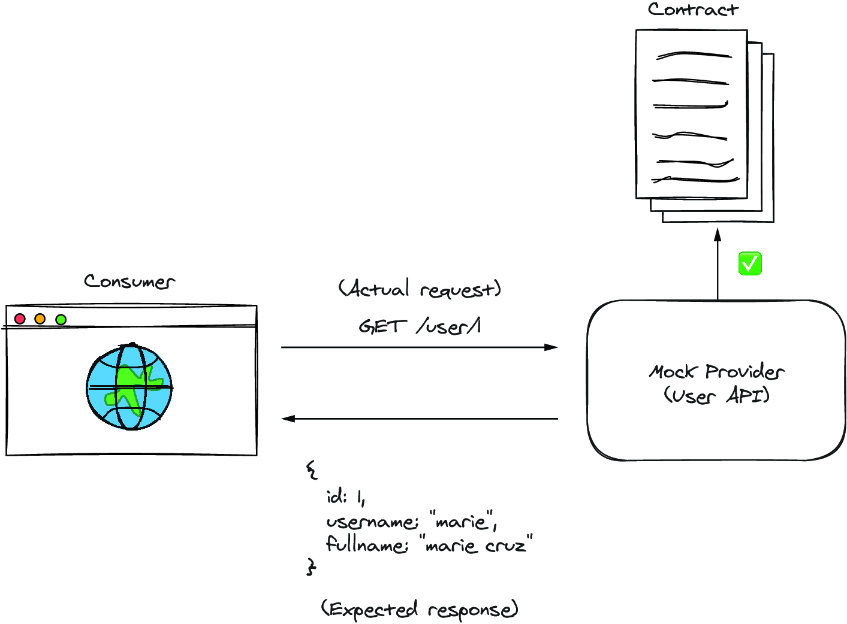
\includegraphics[width=0.8\textwidth]{figures/consumer-side}
    \caption{Ablauf eines Contract Tests auf der Consumer-Seite beim \gls{CDCT}}
    \label{fig:cdct-consumer-side}
\end{figure}

Auf der Provider-Seite wird der Contract dann verwendet, um sicherzustellen, dass die \gls{API} tatsächlich die erwarteten Antworten liefert.
Wie auf der Consumer-Seite kommuniziert der Provider nicht mit dem echten Consumer, sondern mit einem \gls{Mock}-Consumer, der die Anfragen simuliert, um die Unabhängigkeit der Tests zu gewährleisten.
Der Ablauf eines Contract Tests auf der Provider-Seite beim \gls{CDCT} ist in~\cref{fig:cdct-provider-side} dargestellt.
Für jede Anfrage im Contract wird ein Testfall generiert, in dem der \gls{Mock}-Consumer die Anfrage an den Provider sendet.
Der Provider verarbeitet die Anfrage und sendet eine entsprechende Antwort zurück.
Der Test überprüft dann, ob die Antwort des Providers mit der im Contract definierten Antwort übereinstimmt und verifiziert somit, dass die \gls{API} des Providers den Vertrag einhält.

\begin{figure}[ht]
    \centering
    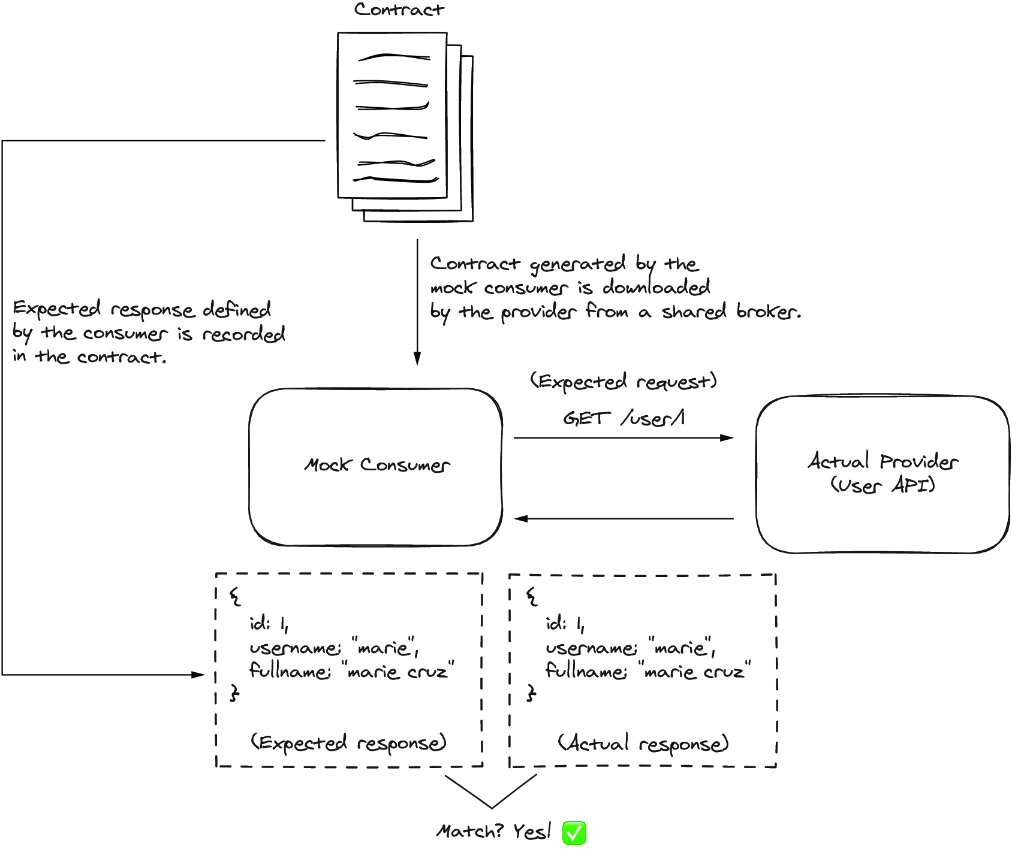
\includegraphics[width=0.8\textwidth]{figures/provider-side}
    \caption{Ablauf eines Contract Tests auf der Provider-Seite beim \gls{CDCT}}
    \label{fig:cdct-provider-side}
\end{figure}

Nun wurde der Contract auf der Consumer-Seite erstellt und auf der Provider-Seite verifiziert.
Das bedeutet, dass beide Seiten unabhängig voneinander auch nach Änderungen in der Zukunft deployt werden können, wenn sie den Contract einhalten.
Dabei können die Tests auf beiden Seiten unabhängig voneinander ausgeführt werden.
Allerdings muss für das Deployen jedes Services sichergestellt werden, dass dazu immer ein verifizierter Vertrag besteht.
Im Umkehrschluss bedeutet das aber auch, dass bei neuen Anforderungen des Consumers an die \gls{API} des Providers auch der Contract aktualisiert werden und vom Provider neu verifiziert werden muss.

Das Verwalten der Contracts ist eine Herausforderung, da es für eine API viele verschiedene Consumer und Versionsstände geben kann.


\subsection{Vor- und Nachteile}\label{subsec:foundation_contracttesting_proscons}
